%acmsmall: The default journal template style.
%acmlarge: Used by JOCCH and TAP.
%acmtog: Used by TOG.
%acmconf: The default proceedings template style.
%sigchi: Used for SIGCHI conference articles.
%sigchi-a: Used for SIGCHI ``Extended Abstract'' articles.
%sigplan: Used for SIGPLAN conference articles.
\documentclass[format=acmtog,12pt,screen=true,review=false,natbib=false,]{acmart}

%% \BibTeX command to typeset BibTeX logo in the docs
%\AtBeginDocument{%
%  \providecommand\BibTeX{{%
%    \normalfont B\kern-0.5em{\scshape i\kern-0.25em b}\kern-0.8em\TeX}}}

%% Rights management information.  This information is sent to you
%% when you complete the rights form.  These commands have SAMPLE
%% values in them; it is your responsibility as an author to replace
%% the commands and values with those provided to you when you
%% complete the rights form.
\setcopyright{acmcopyright}
\copyrightyear{2019}
\acmYear{2019}
\acmDOI{123456789}

%%
%% These commands are for a JOURNAL article.
\acmJournal{TOMACS}
\acmVolume{1}
\acmNumber{1}
\acmArticle{1}
\acmMonth{1}

%%
%% Submission ID.
%% Use this when submitting an article to a sponsored event. You'll
%% receive a unique submission ID from the organizers
%% of the event, and this ID should be used as the parameter to this command.
\acmSubmissionID{123-456-789}

%% Useful packages
\usepackage{multicol}
%\usepackage[UKenglish]{babel}
\usepackage{comment}
\usepackage{textcomp}
\usepackage{tabu}
\usepackage{caption}
\usepackage[scaled]{helvet}
\usepackage[T1]{fontenc}
\usepackage[utf8]{inputenc}
\usepackage{sansmath}
\usepackage{textpos}
\usepackage{ifxetex}
\usepackage{stackengine}
\usepackage{tabularx,longtable,multirow,subfigure,caption} %hang caption
\usepackage{fncylab} %formatting of labels
\usepackage{fancyhdr}
\usepackage{color}

\usepackage{listings}
\usepackage{xcolor}
 
\definecolor{gray}{rgb}{0.4,0.4,0.4}
\definecolor{darkblue}{rgb}{0.0,0.0,0.6}
\definecolor{cyan}{rgb}{0.0,0.6,0.6}

\lstdefinelanguage{XML}
{
  morestring=[b]",
  morestring=[s]{>}{<},
  morecomment=[s]{<?}{?>},
  stringstyle=\color{black},
  identifierstyle=\color{darkblue},
  keywordstyle=\color{cyan},
  morekeywords={xmlns,version,type}% list your attributes here
}
 
 \lstdefinestyle{C}
 {
  belowcaptionskip=1\baselineskip,
  frame=tb,
  numbers=left,
  xleftmargin=\parindent,
  language=C,
  showstringspaces=false,
  basicstyle=\footnotesize\ttfamily,
  keywordstyle=\bfseries\color{green!40!black},
  commentstyle=\itshape\color{purple!40!black},
  identifierstyle=\color{blue},
  stringstyle=\color{orange},
  captionpos=b,
  breaklines=true, postbreak=\mbox{\textcolor{red}{$\hookrightarrow$}\space}
}
\lstset{escapechar=£,style=C}
\usepackage{tcolorbox}
\tcbuselibrary{listings}

\usepackage[ugly]{units}
\usepackage{url}
\usepackage{float}
\usepackage{csquotes}
\usepackage[english]{babel}
\usepackage{amsmath}
\usepackage{bm}
\usepackage{mathtools}
\DeclarePairedDelimiter\ceil{\lceil}{\rceil}
\DeclarePairedDelimiter\floor{\lfloor}{\rfloor}
\usepackage{graphicx}
\usepackage[colorinlistoftodos]{todonotes}
\usepackage{epstopdf} % automatically replace .eps with .pdf in graphics
%\usepackage{backref}
\usepackage{array}
\usepackage{latexsym}
\usepackage{etoolbox}
\usepackage{enumerate} % for numbering with [a)] format 
\usepackage{enumitem}
\usepackage{tablefootnote}
\usepackage{booktabs}
\usepackage{tcolorbox}
\usepackage{silence}
\usepackage{multicol}
%\usepackage{natbib}
\usepackage{multirow}
\usepackage{pbox, cellspace}
\usepackage{tikz}
\usepackage{chemformula}
\let\ce\ch
\usepackage{balance} 
\usepackage{etoolbox}
\usetikzlibrary{shapes,snakes}

\cellspacetoplimit = 6pt
\cellspacebottomlimit = 12pt
\usepackage{seqsplit}
\let\oldseqsplit\seqsplit% Copy \seqsplit
\renewcommand{\seqsplit}{% Redefine \seqsplit to...
  \expandafter\oldseqsplit\expandafter}% ...expand its argument before processing it

\newcommand{\str}[1]{{\ttfamily\seqsplit{#1}}}

\usepackage[style=ACM-Reference-Format,backend=biber,backref=true,hyperref=true,giveninits=true,maxbibnames=999,sorting=none,citestyle=numeric,sortcites]{biblatex} 
\WarningFilter{biblatex}{Patching footnotes failed}

\addbibresource{Bib.bib}
\usepackage{hyperref}
\hypersetup{
  pdftitle={},
  pdfsubject={}, 
  pdfauthor={},
  pdfkeywords={}, 
  pdfstartview=FitH,
  pdfpagemode={UseOutlines},
  bookmarksnumbered=true, 
  bookmarksopen=true, 
  colorlinks=true, 
  citecolor=blue,
  filecolor=blue, 
  linkcolor=blue, 
  urlcolor=blue,
  hypertexnames=true,
  breaklinks=true}

\title[Elementary Implementation of VTK files in C]{Elementary Implementation of VTK XML files}
\subtitle{A FEMDEM Application}

\author{John-Paul Latham}
\authornote{Imperial College London.}
\authornote{Supervisor}
\email{j.p.latham@imperial.ac.uk}

\author{Ado Farsi}
\authornotemark[1]
\authornotemark[2]
\email{ado.farsi@imperial.ac.uk}

\author{Michael Trapp}
\email{mt5918@ic.ac.uk}
\orcid{1234-5678-9012}
\authornotemark[1]

\renewcommand{\shortauthors}{Latham et. al.}

\begin{document}

\begin{abstract}
A recent state-of the arts review by \texttt{EU} decision makers revealed that current building guidelines are not taking into account threats such as natural disasters and acts of terrorism, see \cite{Sto15}. Updating these guidelines requires accurate numerical models to quantify the resilience of building elements against explosive and projectile impact.

The Applied Modelling and Computation Group (\texttt{AMCG}) at Imperial College London has recently developed a novel coupled dynamic gas/solid \texttt{FEMDEM} code.

In this paper, this \texttt{Y} code is applied to simulate \texttt{2D} projectile impact on laminated glass. Furthermore, a novel implementation is presented to prepare and write \texttt{VTK} output files. Before, obsolete external \texttt{VTK} libraries were required to visualise the code output.

The simulation results are not realistic, indicating errors in the preparation software or in the underlying code. The implementation of \texttt{VTK} files is successful and valid output files are produced. The files are visualisable using \texttt{Paraview}. 
\end{abstract}

\begin{CCSXML}
<ccs2012>
<concept>
<concept_id>10010405.10010432.10010439</concept_id>
<concept_desc>Applied computing~Engineering</concept_desc>
<concept_significance>300</concept_significance>
</concept>
</ccs2012>
\end{CCSXML}

\ccsdesc[300]{Applied computing~Engineering}

\keywords{FEMDEM, VTK, Legacy, XML, base64, encoding}

\maketitle

\section{Physics Theory}
\label{sec:PhysicsTheory}

\subsection{Laminated Glass Model}

%Picture of Laminated Glass
%Measurements of the plies and inter-layer

Laminated glass is a sandwich structure of two brittle glass plies and an adhered polymer inter-layer (or inter-face) in between. The bonding between the glass and the inter-layer is without physical adhesive \cite{Sam19}. Secondary laminated glass consists of two such laminates, separated by a layer of air.

\bigbreak
Advantageous properties of laminated glass include a relatively high penetration resistance \cite{Xu14}, low weight \cite{Wu14} and the adherence of fractured glass fragments to the structure to reduce the risk of injuries\cite{Xu14, Che17, Flo98, Ji98}. Breakage of the inner ply significantly reduces strength and facilitates a full collapse of the glass \cite{Flo98}. An optional back layer (usually poly-carbonate (\texttt{PC}) \cite{Bra10, Mon04}) improves structural stability and additional energy absorption \cite{Bio10, Bra10}.

\bigbreak
The prediction of crack initiation and propagation poses a significant challenge and requires ongoing research effort. Local stress intensification is caused by pre-existing micro-structural material flaws (inhomogeneities or discontinuities) such as micro-cracks and voids \cite{Sch12}. 

\bigbreak
Many fracture models have been proposed. The \texttt{Y} code uses a local combined single and smeared crack model approach \cite{Mun99, Lat15}, in which a single crack is replaced by a blunt crack band \cite{Mun04}.

\begin{figure}[!htbp]
    \centering
    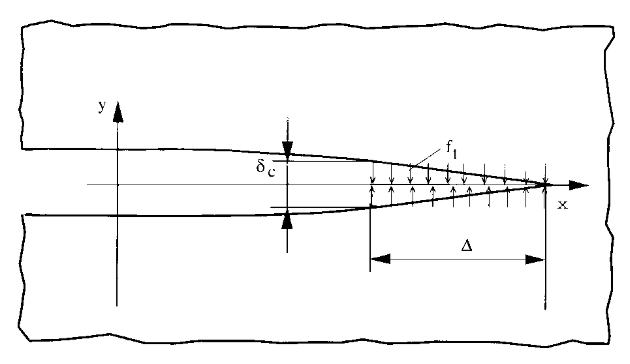
\includegraphics[width=\columnwidth]{IndependentProject/projectplan/Dougale.PNG}
    \caption{Single Crack (Dugdale) Model. \cite{Abu15}}
    \label{fig:dugdale}
\end{figure}

\bigbreak
The single crack model in Fig. \ref{fig:dugdale} assumes a crack tip located in a fracture process zone (\texttt{FPZ}). Plastic bonding stress $\sigma\leq f_{\rm{t}}$ causes the crack tip to open up, up to a critical separation length $\delta=\delta_{\rm{c}}$ \cite{Abu15}. 

\bigbreak
To determine the bonding stress, the \texttt{Y} code adopts the \texttt{Mohr-Coulomb} constitutive model \cite{Lat15}, described by

\begin{equation}
    \label{eq:MohrCoulomb}
    \tau=c+\sigma\,{\rm{tan}}\phi\,,
\end{equation}

with shear stress $\tau$, normal stress $\sigma$, internal cohesion $c$ and internal friction angle $\phi$. The internal friction coefficient is given by

\begin{equation}
    \label{eq:intfriccoeff}
    \eta={\rm{tan}}\phi
\end{equation}

The stresses $\sigma$ and $\tau$ correspond to normal and shear displacements $\delta_{\rm{n}}$ and $\delta_{\rm{s}}$ and tensile and shear strengths $f_{\rm{t}}$ and $f_{\rm{s}}$. These material strengths are defined as the maximum strength in the stress-displacement diagram (Fig. \ref{fig:FractureEnergy}), with maximum elastic displacement $\delta_{\rm{p}}$ and critical displacement $\delta_{\rm{s}}$.

\begin{figure}[!htbp]
    \centering
    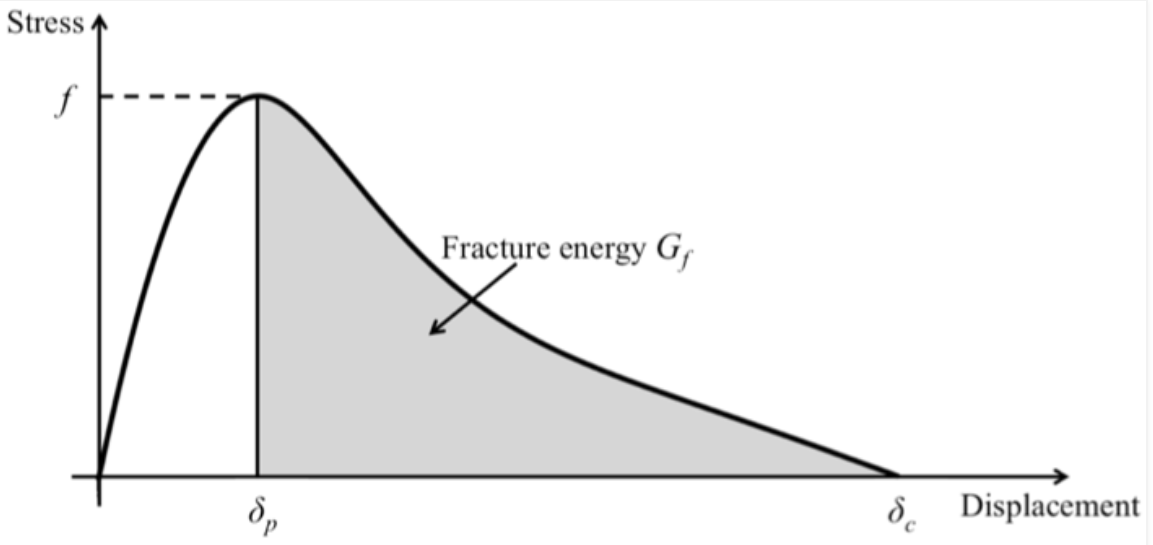
\includegraphics[width=\columnwidth]{FractureEnergy}
    \caption{Stress-displacement curve according to the single and smeared crack model. \cite{Lat15}}
    \label{fig:FractureEnergy}
\end{figure}

The fracturing in the strain-softening part is modelled using joint elements which are generated between two neighbouring shell elements. Cracks coincide with the element edges \cite{Abu15}.

\bigbreak
Further description is given for instance by Latham et al \cite{Lat15}, Munjiza et al \cite{Mun04}, Lei et al \cite{Lei16} and Chen and Chang \cite{Che18}.

\subsection{Inter-layer Model}

The task of the inter-layer is the absorption of impact energy and the maintenance of adhesion to the plies \cite{Wu14}. The inter-layer consists of one or more sheets. Common inter-layer materials include polymers such as polyvinyl butyral (\texttt{PVB}), thermoplastic polyurethane (\texttt{TPU}), and most recently \texttt{SentryGlas}\textregistered Plus (\texttt{SGP}) \cite{Moh18, Wan18}. 

\bigbreak
Mechanical properties of the inter-layer are dependent on the fracture state of the laminated glass \cite{Kun15}. Prior to fracture, straining of the inter-layer is limited, permitting the application of linear visco-elastic laws. After the failure of the glass, the inter-layer is subject to large strains and linear visco-elasticity is no longer applicable. Instead, the inter-layer is modelled as a hyper-elastic material \cite{Gha15, Kim15}. Work done by stresses onto such materials only depends on the reference state $X$ and the current state $x$, but not on the load path (Fig. \ref{fig:deformation}). Deformation from $X$ to $x$ is described by a deformation gradient \cite{Gu07}

\begin{equation}
    \label{eq:defgrad}
    F = \frac{{\rm{d}}\varphi}{{\rm{d}}X}
\end{equation}

with mapping function $\varphi$ mapping from $X$ to $x$.

\begin{figure}[!htbp]
    \centering
    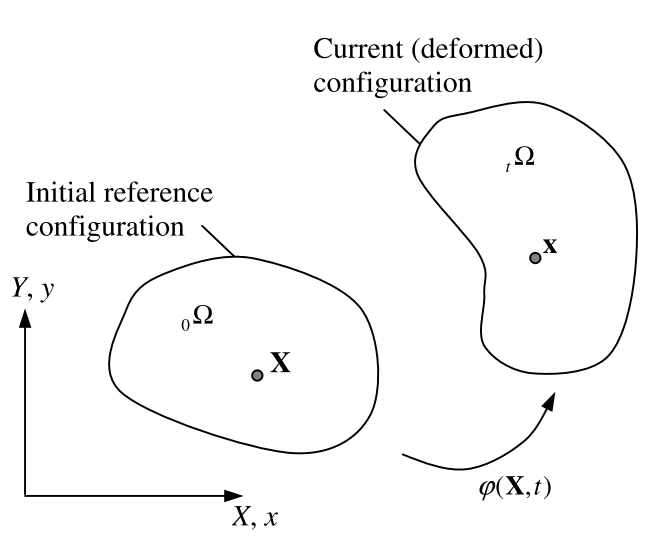
\includegraphics[width=\columnwidth]{Deformation}
    \caption{Deformation from reference to current state. \cite{Gu07}}
    \label{fig:deformation}
\end{figure}

Hyper-elastics are mathematically described by a characteristic strain energy density function $W$. One of the simplest hyper-elastic models is the \texttt{Neo-Hookean} model \cite{Gha15} whose characteristic function is given by

\begin{equation}
    \label{eq:NeoHooke}
    W=\frac{\mu_{\rm{0}}}{2}\left(I_{\rm{1}}-3\right)-\mu_{\rm{0}}\,{\rm{ln}}\,J+\frac{\lambda_{\rm{0}}}{2}{\rm{ln}}^2\,J\,,
\end{equation}

with Lam\'{e} constants $\lambda_{\rm{0}}$ and $\mu_{\rm{0}}$ from the linearised theory, $J=\lvert F\rvert$ and first invariant $I_{\rm 1}=C_{\rm{II}}$ with right Cauchy stress tensor \cite{Gha15}

\begin{equation}
    C_{\rm{ij}}=F_{\rm{Ii}}\,F_{\rm{Ij}}\,.
\end{equation}

Upper case indices refer to the reference configuration, while lower case indices refer to the current configuration.

\bigbreak
Another common, simple hyper-elastic model is the \texttt{Mooney - Rivlin} model \cite{Aba13, Kum16}. The characteristic strain energy function for the compressible 2-Parameter \texttt{Mooney - Rivlin} model \cite{Kum16} is given by

\begin{equation}
    \label{eq:MooneyRivlinSEF}
    W_{\rm{2}} = C_{\rm{10}}\left(\bar{I}_{\rm{1}}-1\right)+C_{\rm{01}}\left(\bar{I}_{\rm{2}}-1\right)+\frac{1}{d}\,(J-1)\,,
\end{equation}

where $C_{\rm{10}}$ and $C_{\rm{01}}$ are adjustable parameters, $d=2\,/\,K$ with bulk modulus $K$ and $\bar{I}_{\rm{1}}=J^{-\frac{1}{3}}\,I_{\rm{1}}$ and $\bar{I}_{\rm{2}}=J^{-\frac{1}{3}}\,I_{\rm{2}}$ are deviatoric invariants \cite{Aba13}. The second invariant is given by

\begin{equation}
    I_{\rm{2}}=\frac{1}{2}\left(C^2_{JJ}-C_{IK}C_{KI}\right)\,.
\end{equation}

\bigbreak
Other hyper-elastic models \cite{Aba13} include a more general polynomial model, \texttt{Arruda-Boyce}, \texttt{Ogden} and \texttt{Yeoh}. For the polynomial model, customized coefficients \cite{Sam19} already exist in the literature, specifically for laminated glass.

\bigbreak
Modelling the occurence of fracture needs to be permitted for the inter-layer as well, as fracturing of the inter-layer is possible. This consideration necessitates the extension of the smeared single and combined fracture model to the inter-layer.

\section{Numerical Modelling Theory}
\label{sec:NumericsTheory}

\subsection{FEMDEM Model}
The combined finite-discrete element method, \texttt{FEMDEM} or \texttt{FDEM}\cite{Wan18, Mun95, Mun99, Mun04, Mun12, Mun13, Guo16, Gao14, Xu14, Che18, Mun13}, contains discrete element that interact with neighbouring discrete elements. In addition, each discrete element is discretised into finite elements. Each finite element mesh captures the deformability of a discrete element. 

\bigbreak
Fracture and fragmentation is modelled as a transition from continua to discontinua. It is also in principle possible to imagine an inverse process of particles merging together.\cite{Mun04}

\bigbreak
Based on the \texttt{3D} \texttt{FDEM} code \texttt{Y3D} by Munjiza et al \cite{Mun95, Mun99, Mun04}, Xiang et al \cite{Xia09} added many detailed improvements and features to the code. The new model, \texttt{Solidity}, is capable of creating realistic coupled multi-physics simulations. In contrast to conventional models, Solidity is not reliant on element deformability restriction constraints (due to the locking problem) and uses simpler triangular, quadratic and tetrahedral elements \cite{Lat15}. 

\subsection{Governing Equations}

The governing equations for the finite element calculations in the \texttt{FEMDEM} method are the equations of motion. The equations are given by

\begin{equation}
    M\ddot{x}+\mu\dot{x}+f_{\rm{int}}=f_{\rm{ext}}=f_{\rm{l}}+f_{\rm{b}}+f_{\rm{c}}\,,
\end{equation}

with lumped nodal mass matrix $M$, nodal displacements $x$, viscosity $\mu$, internal nodal forces $f_{\rm{int}}$ and external nodal forces $f_{\rm{ext}}$. External forces contain consist of external loads $f_{\rm{l}}$, bonding forces $f_{\rm{b}}$ and contact forces $f_{\rm{c}}$. Internal forces $f_{\rm{int}}$ are generated by element deformation. \texttt{FEMDEM} systems solve these equations via explicit time integration using the forward \texttt{Euler} method \cite{Lei16}.

\subsection{Contact Detection}

The combination of discrete and finite elements is established via an interaction algorithm \cite{Lei16}. This algorithm consists of contact detection \cite{Che15} and contact interaction \cite{Mun13}. Contact detection is carried out using search algorithms. 

\bigbreak
The contact detection algorithm detects couples of discrete elements close to each other by eliminating couples of discrete elements that are too far from each other to be in contact. In other words, contact detection avoids processing contact interaction when there is no contact. This reduces \texttt{CPU} requirements and processing run time \cite{Mun04}.

\bigbreak
Contact interaction is only considered for discrete elements which are within a buffer size $b$ of each other, given by

\begin{equation}
    \label{eq:buff}
    b = 0.1\,\Delta_{\rm{min}}\,,
\end{equation}

where $\Delta_{\rm{min}}$ is the minimum edge\footnote{minimum element side length, minimum size}.

\subsection{Contact Interaction}

Penetration of a contractor\footnote{index c} body into a target\footnote{index t} body is implemented in the \texttt{Y} code by the \texttt{potential contact force method}, see Fig. \ref{fig:contact} \cite{Mun04}. Assumption of a conservative force field enables a description of the contact forces using potentials,

\begin{align}
    f_{\rm{c}}^{\rm{2D}}&=-f_{\rm{t}}^{\rm{2D}}=\oint_{\Gamma_{\beta{\rm{t}}\cap\beta{\rm{c}}}}n_{\Gamma}\left(\varphi_{\rm{c}}-\varphi_{\rm{t}}\right)\,{\rm{d}}\Gamma\,,\\
    f_{\rm{c}}^{\rm{3D}}&=-f_{\rm{t}}^{\rm{3D}}=\int_{S_{\beta{\rm{t}}\cap\beta{\rm{c}}}}n_{S}\left(\varphi_{\rm{c}}-\varphi_{\rm{t}}\right)\,{\rm{d}}S\,,
\end{align}

with force potentials $\varphi$ and outward unit normal $n$ to the penetration boundary $\Gamma$ or surface area $S$.

\begin{figure}[!htbp]
    \centering
    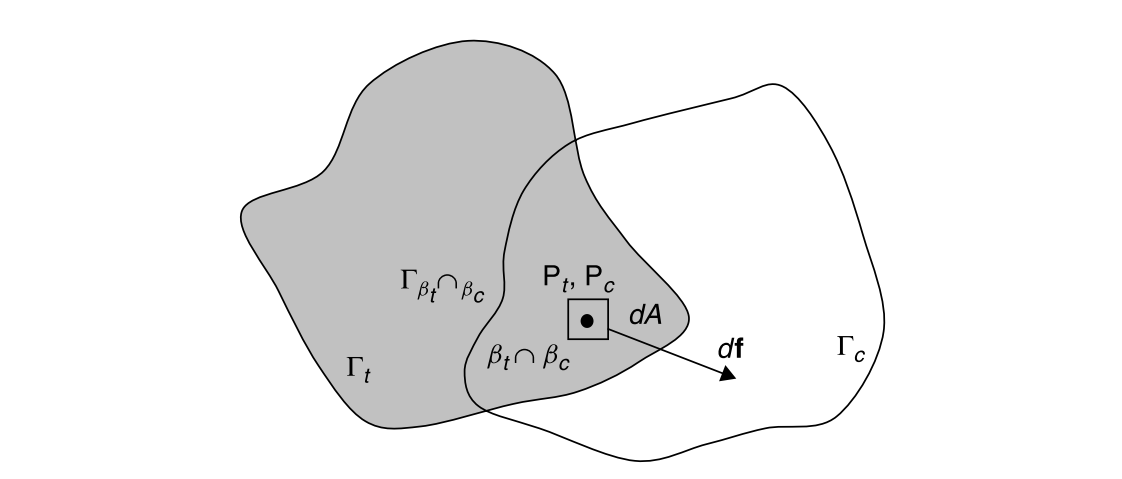
\includegraphics[width=\columnwidth]{Contact}
    \caption{Infinitesimal overlap of contractor and target body. \cite{Mun04}}
    \label{fig:contact}
\end{figure}

\bigbreak
The penetration distance $d$ for each case is given by \cite{Mun04}

\begin{equation}
    \label{eq:d}
    d=\frac{\sigma\,h}{p}\,,
\end{equation}

with applied pressure $\sigma$, element height $h$ and penalty factor $p$. 
\bigbreak
The penalty factor $p$ is given by

\begin{equation}
    \label{eq:p}
    p=\alpha\,E\,,
\end{equation}

with \rm{Young's Modulus} $E$ and a constant $\alpha$ (in this paper: $\alpha=10$) to regulate penetration. 

\bigbreak
Contact damping (Rayleigh damping, viscous damping) due to plastic deformation, breakage of surface asperities, etc. is given by \cite{Mun04}

\begin{equation}
    \label{eq:sigmac}
    \sigma_{\rm{C}}=4\,\xi\frac{\sqrt{p/\rho}}{h}\dot{d}\,,
\end{equation}

\addtocounter{footnote}{-1}
\stepcounter{footnote}
with damping ratio $0\leq\xi\footnotemark\leq1$ and finite element density $\rho$.  

\footnotetext{describes energy dissipation}

\bigbreak
The mass damping coefficient is given by

\begin{equation}
    \label{eq:massdamp}
    \zeta = \sqrt{E\,\rho}
\end{equation}

\section{Numerical Model Approach}
\label{sec:NumericalModelApproach}

\subsection{Workflow}
\label{subsec:SoftwareSetup}

\begin{figure}[h!]
    \centering
    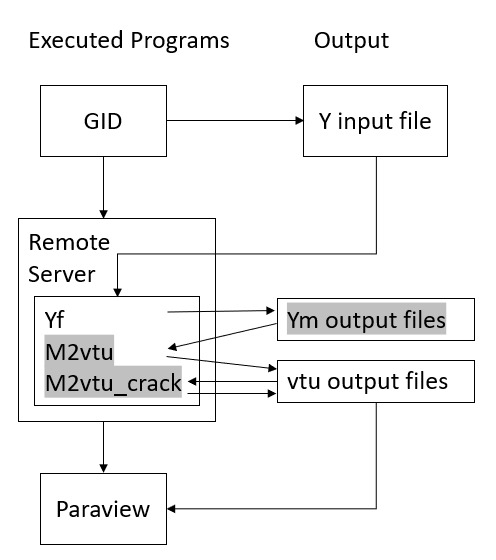
\includegraphics[width=\columnwidth]{Workflow}
    \caption{Workflow of generating a simulation}
    \label{fig:workflow}
\end{figure}

The workflow is illustrated in Fig. \ref{fig:workflow}. The grey shaded items are removed using this paper such that the \texttt{Yf} code now generates the \texttt{VTK} output files directly. The workflow was tested on \texttt{Ubuntu 18.04.2 LTS} subsystem for \texttt{windows 10}.

\bigbreak
A \texttt{2D} input \texttt{Y} file is generated on \texttt{Windows 10} using the open source pre-processor \texttt{CAD} software \texttt{GID} \cite{GID11}. It is possible to instead import the geometry from other \texttt{CAD} software, such as \texttt{AutoCAD}.

\bigbreak
The input file is compiled using three binary files \texttt{Yf}, \texttt{m2vtk} and \texttt{m2vtk\_crack}, which constitute the \texttt{Y2D} code. The program may be obtained from the \texttt{AMCG} at Imperial College London. Code execution requires obsolete \texttt{VTK 5.8} libraries and the obsolete operating system \texttt{Ubuntu 14.4}. Tests were conducted on two remote servers, the high performance computing (\texttt{HPC}) system at Imperial College and a private remote university server.

\bigbreak
The code outputs \texttt{.vtu} files which compose a time series simulation. The output is visualised using the open source software \texttt{Paraview}.

\subsection{Geometry Setup}
\label{subsec:GeometrySetup}

The input file contains the model including the geometry, constraints, materials, as well as the simulation parameters. The majority of modelling parameters are adduced from the literature. A list of material parameters is given in appendix table \ref{tab:matpar}. A list of input file simulation parameters is provided in appendix table \ref{tab:simpar}.

\begin{figure}[h!]
    \centering
    
\includegraphics[width=\columnwidth]{Geometry}
    \caption{\texttt{2D} geometry of the laminated glass structure and projectile \cite{Che18}}
    \label{fig:geometry}
\end{figure}

Fig. \ref{fig:geometry} illustrates the \texttt{2D} geometric setup. The figure shows the initial state of the spherical projectile (yellow) immediately before impact on the laminated glass (impactor glass plies in red, inner glass ply in blue, inter-layer in green). The glass is fixed via a support system (brown). The support structure is not modelled for now and is replaced with no-velocity boundary conditions acting on the sides of the glass plies. 

\bigbreak
In real-world applications, the dimensions of the inter-layer are smaller compared to the glass plies. Therefore, a translational degree of freedom in the \texttt{y}-direction exists for the inter-layer. This effect will also need to be considered in this paper.

\bigbreak
Critical flaws, which cause complete structural failure, are usually found on the cut and machined glass edges \cite{Pel16}. Based on this consideration, the boundary structure layout requires special care. A project task remains to determine a realistic boundary structure to be applied.

\bigbreak
Modifications to this preliminary geometric setup will include changes to the shape of the projectile, as well as changes to the thickness of the layers. A potential consideration is to model the projectile as firearm ammunition instead of a circle (or sphere). A symmetry boundary condition may be applicable and only half of the laminate may need to be modeled.

\bigbreak
The dimensions of the glass plate is set to $2000\,{\rm{mm}}\times2000\,{\rm{mm}}$ in order to avoid anisotropic effects. The thickness of the glass plies is set to $2\,{\rm{mm}}$ and $0.76\,{\rm{mm}}$ for the inter-layer. For now, a \texttt{PVB} material is chosen for the inter-layer.

\bigbreak
The preliminary mesh for all bodies consists of triangular elements. For the \texttt{3D} model, tetrahedral elements \cite{Che18} are to be considered. The preliminary element size is $1\,{\rm{mm}}$. Necessary modifications include reducing the number of elements for the projectile, as it is not of interest for the analysis and increasing the element size for far-field mesh elements for the plies and inter-layer. Potentially, differently shaped elements are more optimal for the results. The glass and inter-layers need to consist of several element layers to enable a more precise analysis. 

\subsection{Material Parameters}
\label{subsec:MaterialParameters}

Table \ref{tab:matpar} lists the material parameters for glass, \texttt{PVB}, steel and rock. The literature provides values for most of the quantities, although they are extremely diverse in some cases. The values used in this paper are marked bold. The elastic and contact penalties are evaluated using Eq. \ref{eq:p}.

\begin{table*}
  \setlength{\tabcolsep}{2pt}
  \small
  %\flushleft
  \caption{List of Y2 input material parameter values.}
  \begin{tabular}{@{}lllll@{}}
    Property & Glass & PVB & Steel Projectile & Rock\tablefootnote{for reference}  \\\midrule
    
    Density $\rho\,\left[{\rm{kg}} / {\rm{m}}^3\right]$
    
                &$2500$ \cite{Xu10, Aba13, Che18, Ved17, Gao14}  
                
                &\begin{tabular}[t]{@{}l@{}}
                    $870$ \cite{Gao14} \\ 
                    $\bm{1100}$ \cite{Xu10, Che18, Ved17} \\
                    $1105{\rm{e}}3$ \cite{Che18}\\
                \end{tabular}
                
                & $7800$ \cite{Che18} & $2700$\\[1em]

    Young's Modulus $E\,\left[{\rm{Pa}}\right]$
    
                & \begin{tabular}[t]{@{}l@{}}
                    $\bm{7{\rm{e}}10}$ \cite{Xu10, Che18, Ved17}\\
                    $7.409{\rm{e}}10$ \cite{Gao14}\\
                    $7.41{\rm{e}}10$ \cite{Che18}\\
                    $7.5{\rm{e}}10$ \cite{Aba13}\\
                \end{tabular}
                
                & \begin{tabular}[t]{@{}l@{}}
                    $\bm{1{\rm{e}}8}$ \cite{Che18} \\
                    $2.2{\rm{e}}2$ \cite{Ved17}\\
                    $5{\rm{e}}10$ \cite{Gao14}\\
                \end{tabular}
                
                & $2{\rm{e}}11$ \cite{Che18} & $3{\rm{e}}10$ \\[1em]
                
    Poisson's Ratio $\nu$ & \begin{tabular}[t]{@{}l@{}}
                                $0.2$ \cite{Che18, Gao14} \\
                                $0.21$ \cite{Aba13} \\
                                $0.3$ \cite{Che18} \\
                                $0.22$ \cite{Xu10} \\
                                $\bm{0.23}$ \cite{Ved17}\\
                                $0.25$ \cite{Che18}
                            \end{tabular}
                          
                          & \begin{tabular}[t]{@{}l@{}}
                                $0.42$ \cite{Che18} \\
                                $0.45$ \cite{Aba13} \\
                                $0.48$ \cite{Gao14} \\
                                $0.49$ \cite{Che15} \\
                                $\bm{0.495}$ \cite{Ved17}
                            \end{tabular}
                          
                          & $0.29$ \cite{Che18} & $0.205$\\[1em]
                          
    Mass damping coefficient $\mu$\tablefootnote{Rayleigh damping, viscous damping} (see Eq. \ref{eq:massdamp}) & $0$ & $0$ & $0$ & $0$ \\[1em]
    
    Elastic penalty term (see Eq. \ref{eq:p}) & $7{\rm{e}}11$ & $1{\rm{e}}9$ & $2.0{\rm{e}}12$  & $3.0{\rm{e}}11$\\[1em]
    
    Contact penalty (see Eq. \ref{eq:p}) & $7{\rm{e}}11$ & $1{\rm{e}}9$ & $2.0{\rm{e}}12$  & $3.0{\rm{e}}11$\\[1em]

    Mode I energy rate $G_{\rm{I}}\,\left[{\rm{J}}/{\rm{m}}^2\right]$ & 
    
    \begin{tabular}[t]{@{}l@{}}
            $\bm{10}$ \cite{Xu10}\\
            $3.9$ \cite{Che18} \\
            $4.0$ \cite{Che18}
        \end{tabular}
        
    & \begin{tabular}[t]{@{}l@{}}
            $2.8{\rm{e}}3$ \cite{Hoo17} \\
            $\bm{20}$ \cite{Che18}
        \end{tabular}  
    
    & $1.9{\rm{e}}5$ \cite{Sta00} & $20.0$\\[1em]

    Mode II energy rate $G_{\rm{II}}\,\left[{\rm{J}}/{\rm{m}}^2\right]$ & $50$ \cite{Xu10} & $2.8{\rm{e}}3$ & $1.9{\rm{e}}5$ & $100.0$ \\[1em]
    
    Mode III energy rate $G_{\rm{III}}\,\left[{\rm{J}}/{\rm{m}}^2\right]$ & $50$ \cite{Xu10} & $2.8{\rm{e}}3$ & $1.9{\rm{e}}5$ & $100.0$ \\[1em]
    
    Tensile Strength $\sigma\,\left[{\rm{Pa}}\right]$ & \begin{tabular}[t]{@{}l@{}}
            $6{\rm{e}}7$ \cite{Che15}\\
            $3{\rm{e}}7$ \cite{Che18}\\
            $\bm{3.46{\rm{e}}7}$ \cite{Che18}\\
        \end{tabular}
        
        & \begin{tabular}[t]{@{}l@{}}
            $\bm{2{\rm{e}}7}$ \cite{Zan12}\\
            $1.862{\rm{e}}7$ \cite{Che18}\\
        \end{tabular}
        
        & $1{\rm{e}}7$ \cite{Wu14} & $4{\rm{e}}6$\\[1em]
        
    Shear Strength $\tau\,\left[{\rm{Pa}}\right]$ & $17.9$ \cite{Che18} & $17.9$ \cite{Che18} & & \\[1em]
    
    Internal friction coefficient $\eta$ (Eq. \ref{eq:intfriccoeff}) & $0.1$ \cite{Che15}  & $0.7$ \cite{Kun15} & $0.15$ \cite{Sah07} & $0.6$ \\[1em]
    
    Internal cohesion $c\,\left[{\rm{Pa}}\right]$ (Eq. \ref{eq:MohrCoulomb}) & $7{\rm{e}}10$ & $2.2{\rm{e}}2$ & $2{\rm{e}}11$ & $8{\rm{e}}6$ \\[1em]
    
    Pore fluid pressure\tablefootnote{\label{notrel}not relevant for glass, \texttt{PVB} and steel} $\left[{\rm{Pa}}\right]$ & $0$ & $0$ & $0$ & $0$ \\
    
    Joint friction coefficient\textsuperscript{\ref{notrel}} & $0.6$ & $0.6$ & $0.6$ & $0.6$ \\
    
    Joint roughness coefficient $\texttt{JRC}_{\rm{0}}$ \textsuperscript{\ref{notrel}, }\tablefootnote{\label{jrc}at laboratory conditions} & $15$ & $15$ & $15$ & $15$ \\
    
    Joint compressive strength $\texttt{JCS}_{\rm{0}}$\textsuperscript{\ref{notrel}, \ref{jrc}} $\left[{\rm{MPa}}\right]$ & $120$ & $120$ & $120$ & $120$ \\
    
    Joint sample size $\left[{\rm{m}}\right]$\textsuperscript{\ref{notrel}} & $0.2$ & $0.2$ & $0.2$ & $0.2$\\[1em]
    
    Interface friction & $0.1$ \cite{Che15} & $0.62$ \cite{Fah07} & $0.44$ \cite{Fah07} & $0.6$ \\
    
    2D Problems & plane strain & & \\\bottomrule
  \end{tabular}
  \label{tab:matpar}
\end{table*}

\subsection{Problem Parameters}
\label{subsec:ProblemParameters}

\begin{table}[t]
  \caption{List of Y2D input simulation parameter values.}
  \begin{tabularx}{\columnwidth}{ll}
    Parameter                               & Value                     \\\midrule
    Maximum number of timesteps $n_{\rm{t}}$ (Eq. \ref{eq:nt})& $2{\rm{e}}6$         \\
    Current number of timesteps             & $0$                       \\
    Restart file saving frequency           & $1{\rm{e}}2$              \\
    Gravity in \texttt{X} Direction (m/s2)  & $0$                       \\
    Gravity in \texttt{Y} Direction (m/s2)  & $0$                       \\
    Gravity in \texttt{Z} Direction (m/s2)  & $-9.8$                    \\
    Timestep (s) (Eq. \ref{eq:deltat})      & $1{\rm{e}}-6$             \\
    Output frequency                        & $2{\rm{e}}3$              \\
    Current number of iterations            & $0$                       \\
    Gravity setting stage (s)               & $0$                       \\
    Load ramping stage (s)                  & $0$                       \\
    Maximum dimension (m)                   & $10$                      \\
    Maximum force (N)                       & $1{\rm{e}}6$              \\
    Maximum velocity (m/s)                  & $100$                     \\
    Maximum stress (Pa)                     & $1{\rm{e}}8$              \\
    Maximum displacement (m)                & $0.1$                     \\
    Minimum joint aperture (m)              & $1{\rm{e}}-7$             \\
    Maximum contacting couples              & $1{\rm{e}}7$              \\
    Buffer Size $b$ for NBS (m) (Eq. \ref{eq:buff})& $7.60{\rm{e}}-5$       \\
    Accuracy (bit)                          & $32$                      \\
    Joint friction model                    & {\small Coulomb}          \\
    Initial aperture correlation            & {\small roughness}        \\\bottomrule
  \end{tabularx}
  \label{tab:simpar}
\end{table}

\begin{table}[t]
  \caption{List of auxiliary parameter values (to calculate simulation parameter values).}
  \begin{tabularx}{\columnwidth}{ll}
    Parameter                               & Value                     \\\midrule
    Total minimum element volume $V_{\rm{e}}$ ($m^3$)& $1.00{\rm{e}}-07$\\
    Total minimum edge $\Delta_{\rm{min}}$ (m)& $4.13{\rm{e}}-04$       \\
    Total real simulation time $t$ (s)        & $10$                    \\
    Critical time step glass (s) (Eq. \ref{eq:deltatcrit})& $2{\rm{e}}6$\\
    Critical time step steel (s) (Eq. \ref{eq:deltatcrit})&$2{\rm{e}}6$ \\
    Critical time step \texttt{PVB} (s) (Eq. \ref{eq:deltatcrit})&$2{\rm{e}}6$   \\
    Overall Mesh size (m)                   & $2.5{\rm{e}}-4$           \\
    Mesh size projectile (m)                & $2.5{\rm{e}}-4$           \\
    Mesh size plies (m)                     & $2.5{\rm{e}}-4$           \\
    Mesh size inter-layer (m)               & $2.5{\rm{e}}-4$           \\\bottomrule
  \end{tabularx}
  \label{tab:simpar}
\end{table}

\bigbreak
The radius of the steel sphere (or circle) is set to $2.5\,{\rm{mm}}$. The critical time step \cite{Far19}\footnote{\label{DEMPlus} for inquiries concerning this reference please contact the \texttt{AMCG} at Imperial College London} is set accordingly to

\begin{equation}
\label{eq:deltatcrit}
\Delta t_{\rm{crit}}=\sqrt{\frac{V_{\rm{e}}\footnotemark\,\rho\footnotemark}{p}}=\sqrt{\frac{0.000413\cdot7.8\cdot10^3}{4\cdot{10}^{11}}}{\rm{s}}\,.
\end{equation}

\addtocounter{footnote}{-2}
\stepcounter{footnote}
\footnotetext{volume  $\left({\rm{in}}\,{\rm{m}}^3\right)$ of the smallest finite element, without units}
\stepcounter{footnote}
\footnotetext{density $\left({\rm{in}}\,{\rm{kg}}/{\rm{m}}^3\right)$ of the material of the smallest finite element, without units}

The acceptable time step $\Delta t$ is given by

\begin{equation}
    \label{eq:deltat}
    \Delta t= \floor{\Delta t_{\rm{crit}}} = 3\rm{e}-6{\rm{s}}\,,
\end{equation},

where $\floor{\,}$ denotes the floor operator. To simulate real time $t=10\,{\rm{s}}$, the maximum number of time steps required \cite{Far19}\textsuperscript{\ref{DEMPlus}} is given by

\begin{equation}
    \label{eq:nt}
    n_{\rm{t}}=\frac{t}{\Delta t}=\frac{10\,{\rm{s}}}{3\,{\rm{e}}-6\,{\rm{s}}}=1{\rm{e}}6\,.
\end{equation}


\subsection{Verification}
\label{subsec:Verification}

Meeting specified accuracy standards \cite{Sto15} requires verification of the numerical model by use of data from numerical experiments. Physical experiments involving the breakage of glass by projectiles or shock blasts require special safety arrangements. Air blast impact experiments are being conducted outdoors by service company \texttt{Jabisupra} \cite{Jab16} in cooperation with Imperial College London. The company is active in the field of envelope security and specialises in protecting infrastructure from certain threats. The data from \texttt{Jabisupra} is not expected to yet be ready and applicable for this project. Many other researchers have already conducted impact experiments in the past and a majority of the findings from these experiments are likely to be applicable to verify the model for this project.

\bigbreak
Dynamic impact on laminated glass comprises hard and soft body impact \cite{Moh17}. Hard body impact such as ballistic impact \cite{Bra10} causes minimal deformation to the projectile, while soft body impact such as bird impact \cite{Moh17} causes the projectile to undergo extensive deformation.

\bigbreak
Relevant parameters of the impact projectile include the normal velocity \cite{Gra98, Kar14, Dar13, Wu14}, the mass \cite{Kar14, Dar13}, the angle \cite{Gra98, Kar14, Dar13}, the shape \cite{Dar13} and the size \cite{Wu14}. Relevant parameters for the outer glass ply include its dimensions \cite{Wan18}, its mass, the support conditions \cite{Wan18} and the make-up \cite{Wan18}. For the inter-layer, the material \cite{Moh18, Wan18, Mon04}, thickness \cite{Ji98, Kar14, Wan18} and temperature \cite{Moh18, Zha19} are relevant.

\bigbreak
Low velocity ($\approx 20\,\mathrm{m}/\mathrm{s}$) hard impact experiments include the use of projectiles in form of road construction chippings \cite{Gra98}, ballistics \cite{Mon04}, drop-down weights \cite{Che15, Mil12, Wan18}, aluminum projectiles \cite{Mil12} and steel balls \cite{Beh99, Flo98, Wan18}. High velocity (around $180\, {\rm{m}}/{\rm{s}}$) soft impact experiments include the use of silicon rubber projectiles \cite{Moh17} and gas guns \cite{Moh18}.

\bigbreak
Wang et al \cite{Wan18} found that the panel size had an inferior effect on the breakage resistance \cite{Wan18}. Similarly, Monteleone et al \cite{Mon04} found that only a local area of the ply around the impact absorbed the impact energy for high velocities.

\bigbreak
Karunarathna \cite{Kar14} found that impact velocity and plate thickness contributed significantly towards the impact resistance, compared to impact mass and inter-layer thickness. Wang et al \cite{Wan18} found an increased inter-layer thickness to have a negative effect on energy absorption. Liu et al \cite{Liu16} established that the inter-layer thickness did not contribute towards energy absorption. Behr and Kremer \cite{Beh99} found an increased inter-layer thickness to better protect the inner ply. Kim et al \cite{Kim16} numerically optimised the \texttt{PVB} inter-layer constitution to prevent all damage to the inner glass ply.

\bigbreak
Liu et al \cite{Liu16} numerically investigated the optimisability of the inter-layer in terms of energy absorption by simulating the impact of a human head. Zhang et al \cite{Zha19} investigated the influence of temperature on the inter-layer and found that a hybrid \texttt{TPU}/\texttt{SGP}/\texttt{TPU} inter-layer performed best over the entire range of tested temperatures.

\section{Computer Science Approach}
\label{sec:ComputerScienceApproach}

The following definitions are adopted from the code:

\begin{lstlisting}[language=C, caption=Data type definitions, label=lst:definitions]
#define FLT float
#define INS int
#define DBL double
#define INT long
#define UCHR unsigned char
#define CHR char
#define UINT unsigned int
#define ULON unsigned long
\end{lstlisting}

\subsection{VTK format}
\label{subsec:VTKformat}

The Visualisation Toolkit \texttt{VTK} \cite{Kit} is an extremely popular open source software for graphic visualisation of scientific data. \texttt{VTK} \texttt{API}s are available in many different programming languages and facilitate the generation of \texttt{VTK} files. Until now, the \texttt{Y} code used the \texttt{C} programming language \texttt{VTK} \texttt{API} to generate simulation output. 

\bigbreak
The required \texttt{VTK} version \texttt{5.8} library dependencies revealed themselves to be outdated and unobtainable. This limited the applicability of the entire \texttt{Y} code to operating systems which support this obsolete version. Specifically, all attempts by the author to obtain such a version for testing were not successful. Rewriting the code using a newer \texttt{VTK} version would only temporarily solve the problem.

\bigbreak
To diversify application to a wider range of operating systems, it was deemed necessary to hard code the output with eschewal of \texttt{VTK} libaries. Aside from the partly ill-documented offical website \cite{Kit}, one of the only few reliable resources available is the \texttt{Earth Models} website by Bunge \cite{Bun09}. In what follows, the aim is to provide the reader with a more detailed and more in-depth description of the \texttt{VTK} format. 

\subsection{VTK legacy file format}
\label{subsec:VTKlegacyfileformat}

The \texttt{VTK} legacy file format is sufficiently documented (see \cite{Kit} for official documentation) and relatively easy to implement. On the downside, it only supports a minimal amount of features and is relatively inflexible. List. \ref{lst:vtklegacy} shows an example \texttt{VTK} legacy file. 

\bigbreak
The header defines \texttt{VTK} version, file name, data encoding (\texttt{ascii} or \texttt{binary}) and dataset type \footnote{here: unstructured grid} \cite{Kit}.

\bigbreak
The data is divided into sections including points, cells, cell types. The section header contains the keyword along with the total amount of entities of the section. The data is written continuously using spaces as separators. \cite{Kit}

\bigbreak
Every section has additional unique formatting rules. The points sections requires an additional data type identifier (here: \lstinline{float}) to correctly identify the coordinates data. \cite{Kit}

\bigbreak
The data in the cells section lists the node numbers of each element, appended to a number identifying the total amount of nodes of the element. \cite{Kit}

\bigbreak
The cell type section identifies the geometric shape of each element, given by an index. Each index is written on a separate line. \cite{Kit}

\subsection{VTK XML file format}
\label{subsec:VTKXMLfileformat}

Compared to \texttt{legacy} files, \texttt{XML} files are much more difficult to implement. An example is given in List. \ref{lst:vtkxmlinline}. 

\bigbreak
The file is structured using nested keyword headers which are enclosed in angle brackets ("<" and ">"), according to \texttt{XML} language. Text indentation is not required but enhances readability.

\bigbreak
Keyword headers are opened using \lstinline[language=XML]{<keyword>} and closed using \lstinline[language=XML]{</keyword>}. Keywords which do not contain any sub-keyword headers are opened and closed in one line using \lstinline[language=XML]{<keyword\>}. Keyword headers usually contain additional mandatory and optional keywords in the format of \lstinline[language=XML]{option="value"} \cite{Kit}.

\bigbreak
The file header specifies versions, \texttt{VTK} file type and \lstinline[language=XML]{byte_order} \footnote{endianess, here: little endian} \cite{Kit}. Big endian byte order was not tested, as such operating systems were not available for testing.

\bigbreak
Depending on the specified \lstinline[language=XML]{VTKFile type}, a unique set of sub-keyword headers is used. For the \lstinline[language=XML]{Unstructured_Grid} \texttt{VTK} file type chosen here, the file content is structured using \lstinline[language=XML]{<Piece>}. Within this header, it is required to specify the number of points and cells (elements) using \lstinline[language=XML]{NumberOfPoints} and \lstinline[language=XML]{NumberOfCells} \cite{Kit}.

\bigbreak
\lstinline{<Piece>} contains definition of \lstinline[language=XML]{<Points>} and \lstinline[language=XML]{<Cells>}, among other optional keyword sub-headers. \lstinline[language=XML]{<Points>} expects exactly one \lstinline[language=XML]{<DataArray>} containing the nodal coordinates. \lstinline[language=XML]{<Cells>} expects one \lstinline[language=XML]{<DataArray>} each for the cell connectivity (node configuration of each cell), the cell offsets (offsets in the cell connectivity list), as well as the cell type (cell shape index, see \cite{Kit}) \cite{Bun09}.

\bigbreak
The data, listed after \lstinline[language=XML]{<DataArray>} includes \lstinline[language=XML]{type} (data type), \lstinline[language=XML]{Name}, \lstinline[language=XML]{NumberOfComponents}, \lstinline[language=XML]{format}, \lstinline[language=XML]{RangeMin} and \lstinline[language=XML]{RangeMax}.

\bigbreak
\lstinline[language=XML]{RangeMin} and \lstinline[language=XML]{RangeMax} indicate the minimal and maximal values of the data and are optional\footnote{confirmed by tests}. Simple array search functions were implemented in order to find the individual values.

\bigbreak
\lstinline{Name} specifies a unique name, enclosed by \texttt{""}, for the data set. The data array contained in \lstinline[language=XML]{<Points>} requires no name. The data arrays enclosed by \lstinline[language=XML]{<Cells>} require fixed names \lstinline[language=XML]{Name="connectivity"}, \lstinline[language=XML]{Name="offsets"} and \lstinline[language=XML]{Name="types"} \cite{Kit}.  

\bigbreak
\lstinline[language=XML]{format} specifies the encoding of the data.

\bigbreak
In the case \lstinline{format="ascii"}, the data is provided in decimal form, delimited by spaces, similar to section \ref{subsec:VTKlegacyfileformat} \cite{Bun09}. Specifying an inappropriate data \lstinline[language=XML]{type} for this format will not leave the data completely unusable, although induced type casting may yield unexpected results. The dependence on spaces as delimiters is highly impractical when transferring files between different operating systems and applications. 

\bigbreak
A more robust option is given by \lstinline{format="binary"}. Characters such as "<" (binary encoding of 0b00111100=d060) may potentially appear in binary encoded data. As these characters compose \texttt{XML} keyword headers, binary encoding is not realizable \cite{Bun09}. Thus, the data is encoded to \texttt{base 64} (\texttt{b64}) (see \ref{subsec:b64encoding}). 

\bigbreak
For \texttt{b64} encoding, a data header needs to be prepended to the data. The data header is always of type \lstinline[language=C]{int32} (data size: 4 bytes) and specifies the data size, i.e. the amount of binary bytes of subsequent data. The data size is not to be confused with the length of the printed \texttt{b64} encoded data string in the output file, which is insignificant for now. The data size rather refers to the size of the binary data array in \lstinline[language=C]{bytes}, stored as specified by the datatype in the header. Specifying a data \lstinline[language=XML]{type} of a different \texttt{byte} size for this format produces errors and renders the data useless.

\bigbreak
As an example, consider a \lstinline[language=C]{float32} array which contains $100$ data values. The corresponding header is given by:

\begin{equation}
\label{eq:b64inlineex}
    h=100\,\frac{32\,{\rm bits}}{8\,{\rm bits}/{\rm byte}}=400\,{\rm bytes}
\end{equation}

\bigbreak
The header then needs to be encoded to b64, separately from the data. The encoded header string is immediately followed by the encoded data string, without any delimiters. Considering the fact that the data header type is fixed, the \texttt{b64} encoded data header string length is always the same. Thus, no additional offset is necessary to specify the positional onset of the data after the data header \cite{Bun09}.

\bigbreak
Instead of supplying the data inline, it is possible to append data once, to an \lstinline{<AppendedData>} section at the end of the file. This is achieved by specifying option \lstinline[language=XML]{format="appended"} for each data array keyword header and providing an \lstinline[language=XML]{offset} each time.

\bigbreak
In doing so, the entire data is provided in a single long \texttt{b64} encoded string, appended to an underscore "\_". Like in the inline format, each encoded data string must be prepended by a \texttt{b64} encoded header, which specifies the size of the following unencoded data section in bytes. The headers and the data sections are encoded separately each, without any delimiters between headers and data sections.

\bigbreak
The offset value provided in each \lstinline[language=XML]{<DataArray>} specifies the amount of bytes of unencoded data after the underscore to the beginning of the corresponding header. The method of evaluation of header offsets is illustrated in Tab. \ref{tab:offset}.

\begin{table*}[t]
  \caption{Breakdown of offset values for an example output file with $642$ points and $1280$ cells. The desired (header) offsets are given in column $2$.}
  \begin{tabular}{@{}llllllll@{}}
    Name & header offset & data offset & data size & data type size & values & components & points/cells \\\midrule
    Points & 0 & 4 & 15408 & 8 & 1926 & 3 & 642\\
    Connectivity & 15412 & 15416 & 15360 & 4 & 3840 & 3 & 1280\\
    Offsets & 30776 & 30780 & 5120 & 4 & 1280 & 1 & 1280\\
    Types & 35900 & 35904 & 1280 & 1 & 1280 & 1 & 1280\\
    Points s & 37184 & 37188 & 5136 & 8 & 642 & 1 & 642\\
    Points v & 42324 & 42328 & 15408 & 8 & 1926 & 3 & 642\\
    Points n & 57736 & 57740 & 15408 & 8 & 1926 & 3 & 642\\
    Density & 73148 & 73152 & 5136 & 8 & 642 & 1 & 642\\\bottomrule
  \end{tabular}
  \label{tab:offset}
\end{table*}

\bigbreak
In Tab. \ref{tab:offset}, the header offset of the first header is always $0$. As the unencoded header is always an \lstinline[language=C]{int32} of size $4\,{\rm bytes}$, the first data offset is $4$. For a data array with $1926$ values and data type size $8\,{\rm bytes}$ (e.g. \lstinline[language=C]{float64}), the data size in \lstinline[language=C]{bytes} amounts to $1926\cdot8\,{\rm bytes}=15408{\rm bytes}$. The number of values is comprised by the number of components and the number of points, i.e. $3\cdot642=1926$. The next header offset is evaluated by adding the data size to the data offset, i.e. $4+15408=15412$. The remaining offset values are evaluated accordingly.

\subsection{Base 64 encoding}
\label{subsec:b64encoding}

%\begin{figure}
%\begin{tikzpicture}
% \draw (0,0) node[anchor=north] {float* array}
% \draw (2,0) node[anchor=north] {float}
% \draw (4,0) node[anchor=north] {float byte}
%\node [rectangle split,rectangle split parts=36, rectangle split vertical,draw ] %at (0,0);
%\node [rectangle split,rectangle split parts=32, rectangle split vertical,draw ] %at (0,0);
%\node [rectangle split,rectangle split parts=32, rectangle split vertical,draw ] %at (2,0);
%\node [rectangle split,rectangle split parts=8, rectangle split vertical,draw ] %at (2,0);
%\node [rectangle split,rectangle split parts=8, rectangle split vertical,draw ] %at (2,-1);
%\node [rectangle split,rectangle split parts=8, rectangle split vertical,draw ] %at (2,-2);
%\node [rectangle split,rectangle split parts=8, rectangle split vertical,draw ] %at (2,-3);
%\end{tikzpicture}
%\caption{Data segmentation of a \lstinline{float*} array. Each rectangle %represents one bit in memory.}
%\label{fig:segmentation}
%\end{figure}

The output data consists of one- and two-dimensional \lstinline{int} and \lstinline{float} arrays containing nodal properties, elemental properties and flags. The computer stores the data in binary form, according to byte order (endianess) of the operating system at hand.

\bigbreak
\lstinline{float} numbers are usually stored in \texttt{IEEE-754} format \cite{Asp14}. As the numbers are stored internally, the exact manner of storage is theoretically not significant as long as the position (the significance) of the bits in binary-stored \lstinline{float} is not being violated.   

\bigbreak
As the base64 encoding function takes in a contiguous \lstinline{CHR*} array, the data needs to be segmented into bytes. For the \lstinline{INS} data header, this simply involves conversion from a 4-byte \lstinline{int32} to 4 \lstinline{CHR} bytes. The segmentation process for arrays is illustrated in Fig. \ref{fig:b64}. The array is segmented into single bytes, rearranged in groups of 3 bytes and again rearranged in groups of 6 bits. The 6-bit groups are encoded to characters and compose the encoded string. 

\bigbreak
As an example, the implementation approach is discussed by use of the 2-dimensional contact force array. A complete implementation can be found in file \lstinline{Yod.c}. In a first step, 2-dimensional arrays are reduced to contiguous one-dimensional arrays (List. \ref{lst:2d21d}).

\begin{lstlisting}[language=C, caption=Converting 2-dimensional array to 1-dimensional array for contiguity, label=lst:2d21d]
DBL *cf; //contact force
INS i, j, k;
INS header;
header = sizeof(DBL) * ydn->nnopo * ydn->nnodim;
cf = malloc(header);
k = 0;
for (i = 0; i != ydn->nnopo; i++){
  for (j = 0; j != ydn->nnodim; j++){
    cf[k] = ydn->d2nfcon[j][i];
    k++;}
  cf[k] = ydn->d2nfcon[j][i];
  k++;}
\end{lstlisting}

In List. \ref{lst:2d21d}, \lstinline{ydn->nnopo} denotes, in the class "\textbf{Y} \textbf{d}atabase of \textbf{n}odes", the current \textbf{n}umber of \textbf{nodal} \textbf{po}ints. \lstinline{ydn->nnodim} denotes the current \textbf{n}umber of \textbf{no}dal \textbf{dim}ensions (2) and \lstinline{ydn->d2nfcon} denotes the \textbf{d}ouble \textbf{2}-dimensional \textbf{n}odal \textbf{f}orce of \textbf{con}tact. 

\bigbreak
As a result, the data is now stored in a contiguous one-dimensional array of \lstinline{float64} and now needs to be segmented into bytes.
\begin{figure}[!htbp]
    \centering
    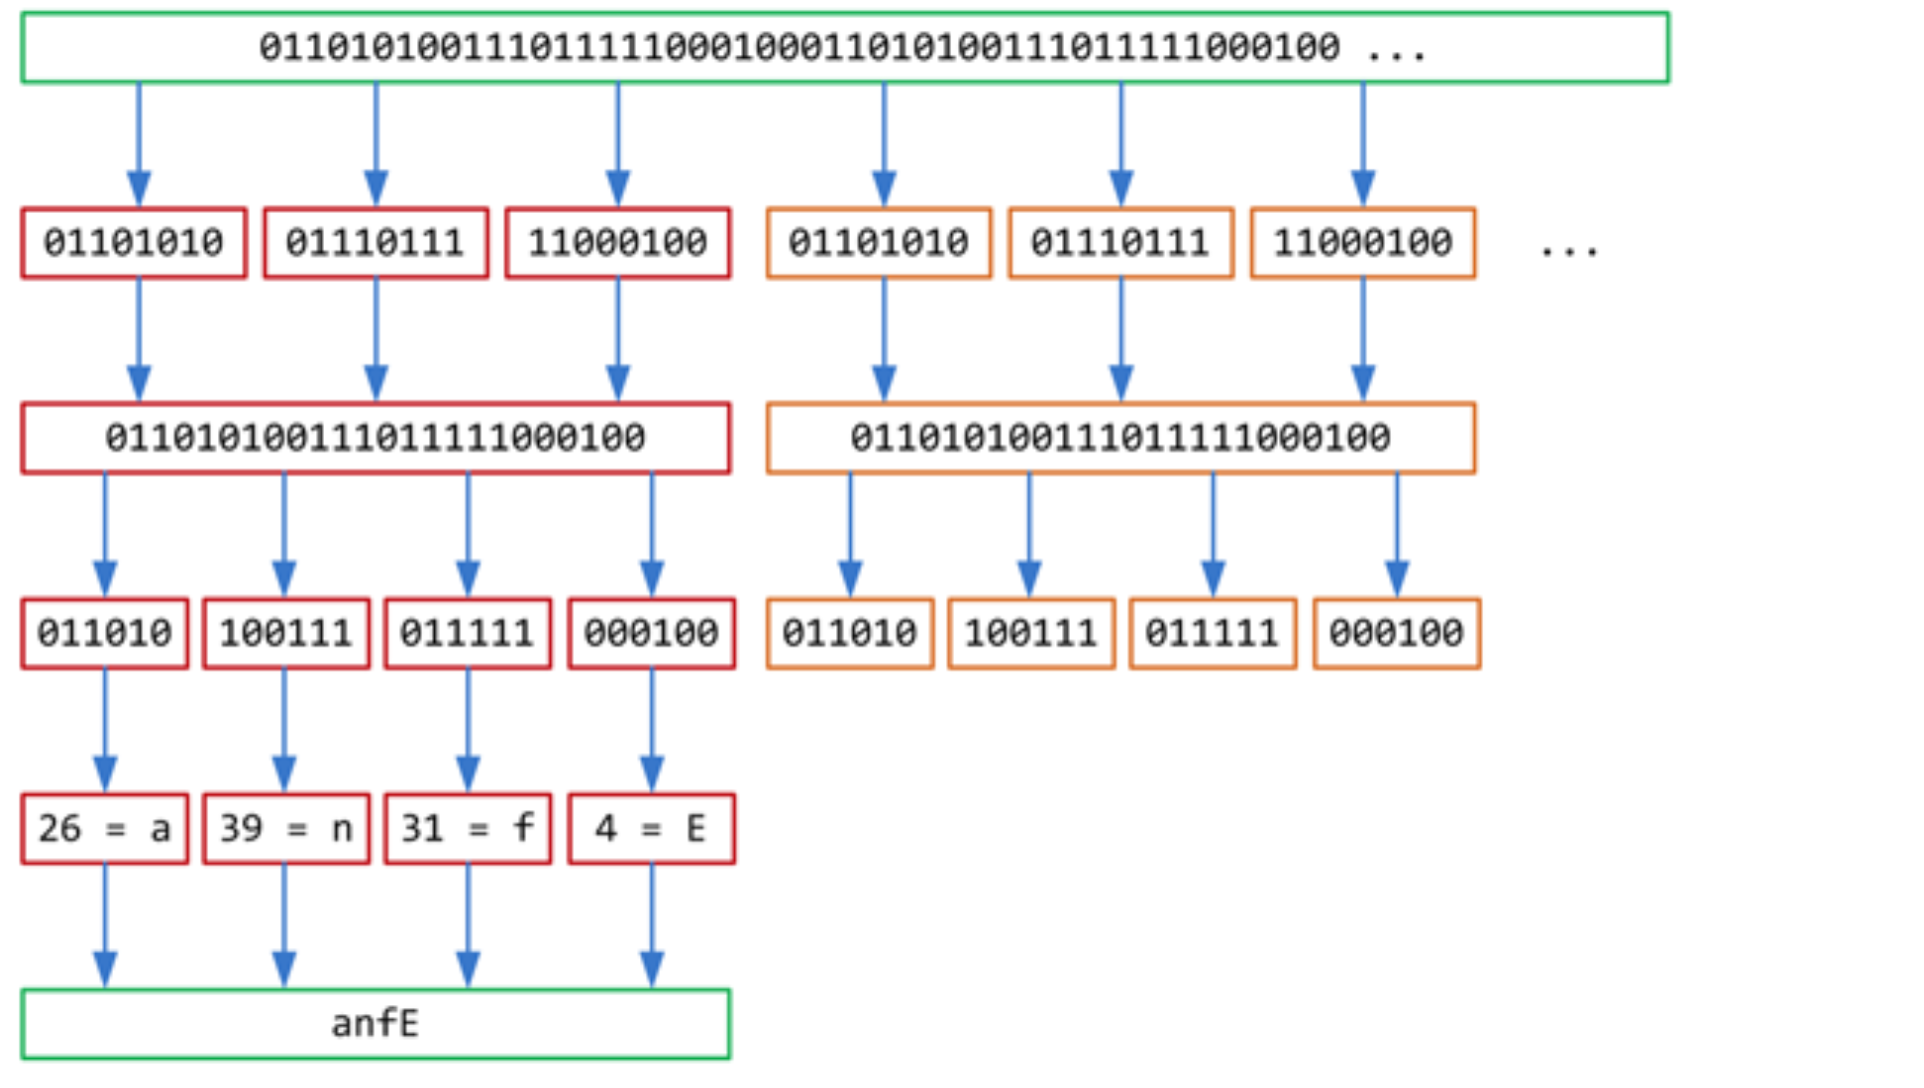
\includegraphics[width=\columnwidth]{b64}
    \caption{Subsequent conversion of binary data to bytes, bit sextets, and encoded characters \cite{App}.}
    \label{fig:b64}
\end{figure}

A first possible strategy is to apply simple data type casting, see List. \ref{lst:typecasting}.

\begin{lstlisting}[language=C, caption=Segmentation approach via type casting with pointers, label=lst:typecasting]
FLT floats[4] = {1, 2, 3, 4}
//actual array is of variable size;
CHR *bytes = (CHR *) floats;
\end{lstlisting}

The \lstinline{CHR* bytes} array could then be passed on to the encoding function. Test showed that this strategy seems to only work if the array to type cast does not contain any data before type casting. Thus, this approach is not appropriate here.

\bigbreak
A second possible strategy is to declare a \lstinline{union}, see List. \ref{lst:union}.

\begin{lstlisting}[language=C, caption=Segmentation approach via a union, label=lst:union]
union INTToCHR {
  INS i;
  CHR *c[sizeof(INS)];};
\end{lstlisting}

Here, both \lstinline[language=C]{i} and \lstinline[language=C]{c} refer to the same location in memory. This approach potentially works for a single \lstinline[language=C]{float}. As the \lstinline[language=C]{CHR*} arrays would need to be concatenated dynamically, this approach is (according to the author's opinion) not appropriate either. Test which were carried out using this strategy showed inconsistent outputs, indicating that the prompted data may not be contiguously stored.

\bigbreak
A third strategy for dividing the data arrays into bytes uses a combination of \lstinline[language=C]{malloc} and \lstinline[language=C]{memcpy}.

\begin{lstlisting}[language=C, caption=Segmentation approach via memcpy, label=mallocandmemcpy]
CHR *bytes;
bytes = malloc(header);
memcpy(&bytes[0], cf, header);
\end{lstlisting}

Testing confirmed that this method is successful. The \lstinline[language=C]{byte} array now contains the floats in contiguous order in binary form, stored as bytes. 

\bigbreak
The prepared data is passed to the base 64 encoding function \lstinline[language=C]{b64enc} in file \lstinline[language=C]{Yod.c}. The function takes some \lstinline[language=C]{CHR*} array \lstinline[language=C]{src} of length \lstinline[language=C]{len} as input, encodes it byte for byte and outputs character for character into the \texttt{VTK} output file \lstinline[language=C]{fout}. 

\bigbreak
The core of the algorithm (List. \ref{lst:b64alg}) was adopted from Malinen \cite{Mal05}.

\begin{lstlisting}[language=C, caption=b64 algorithm, label=lst:b64alg]
while (end - in > 2){
  putc(enc[in[0] >> 2], fout);
  putc(enc[((in[0] & 0x03) << 4) | (in[1] >> 4)], fout);
  putc(enc[((in[1] & 0x0f) << 2) | (in[2] >> 6)], fout);
  putc(enc[in[2] & 0x3f], fout);
  in += 3;}
  
if (end - in){
  putc(enc[in[0] >> 2], fout);
  if (end - in == 1){
    putc(enc[(in[0] & 0x03) << 4], fout);
    putc('=', fout);}
  else{
    putc(enc[((in[0] & 0x03) << 4) | (in[1] >> 4)], fout);
    putc(enc[(in[1] & 0x0f) << 2], fout);}
  putc('=', fout);}
return;}
\end{lstlisting}

In List. \ref{lst:b64alg}, \lstinline{in} and \lstinline{end} are \lstinline{CHR*} pointers which point to the beginning and end of the input array. Converting to base 64 requires rearranging the input in chunks of 6 bits. Each of these 6-bit chunks produces a value $\varv < 64 = 0b1000000$ and is able to be converted to one of 64 unique characters from the encoding array \lstinline{CHR* enc = "ABCDEFGHIJKLMNOPQRSTUVWXYZabcdefghijklmnopqrstuvwxyz0123456789+/"}. 

\bigbreak
For every $3$ bytes (or $24$ bits), the algorithm produces $4$ groups of $6$ bits, i.e. $4$ characters. The bits are extracted continuously via bit shifting. As mentioned before, the position or significance of the bits in the byte must not be violated. In other words, the value of the bit must not get lost through bit shifting. The algorithm is now explained in detail: 

\bigbreak
In line $2$, the first $6$ bits of the current character \lstinline{in[0]} are extracted by bit shifting to produce the first $6$-bit chunk. The value of this chunk is used to produce the index of the corresponding character in the encoding array \lstinline{enc}. 

\bigbreak
The last two remaining bits of the current input character \lstinline{in[0]} are evaluated and bit shifted in line $3$ to account for the first $2$ significant bits of the next $6$-bit chunk. The $4$ missing bits to complete the $6$ bits are extracted from the first $4$ bits of the second character \lstinline{in[1]}, again by bit shifting.    

\bigbreak
In line $4$, the $4$ remaining bits from the second input character \lstinline{in[1]} make up the first four bits of the next $6$-bit chunk. The missing $2$ bits of the $6$-bit chunk are extracted from the third input character \lstinline{in[2]}. This leaves $6$ bits of the third input character remaining, making up another $6$-bit chunk, as implemented in line $5$.

\bigbreak
If the input array length \lstinline{len} = \lstinline{end} - \lstinline{in} is not divisible by $3$, padding characters are required. The amount of padding padding depends on the amount of remaining input byes to complete a group of three input bytes. If $\rm{len}\,\%\,3==1$, two padding characters '==' are appended to the encoded string. If $\rm{len}\,\%\,3==2$, one padding character '=' is required. The algorithm is given in List. \ref{lst:b64alg}, lines 8-17.

\section{Results}

\subsection{Simulation}

\subsection{VTK implementation}

\lstinputlisting[language=XML, caption=Example vtk legacy file, label=lst:vtklegacy]{IndependentProject/finalreport/vtk_legacy.vtu}

\lstinputlisting[language=XML, caption=Example vtk xml file with inline encoding file, label=lst:vtkxmlinline]{IndependentProject/finalreport/vtk_xml_inline.vtu}

\section{Discussion}

\subsection{Simulation}

The simulation results are not realistic. The projectile of prescribed material steel locally deforms on impact on the glass, while the glass ply does not show any reaction to the impact.

\bigbreak
A likely cause might be implementation issues in the pre-processing softwares. The pre-processors \texttt{GID} and \texttt{AutoCAD} proved to be extremely unreliable. The input file prepared using \texttt{GID} contained contradictory definitions compared to the code. For example, the nodes which make up each element were defined in oppose rotational direction \texttt{GID}. It may be possible that importing geometries from \texttt{AutoCAD} produced this error. Another possibility may the that the preprocessor may produce different output on different operating systems. As code for these programs is not publicly available, further investigation is not possible.  

\bigbreak
Another plausible cause might be errors in the code. The code cannot be executed in a clean environment, such as the \texttt{Travis} environment in a \texttt{Github} repository. Specifically, the error occurs at the beginning of the program in line $733$ in file \lstinline{Yrd.c}, see List. \ref{lst:setlinebuferror}.

\begin{lstlisting}[language=C, caption=\lstinline{SETLINEBUF} Error in file \lstinline{Yrd.c},label=lst:setlinebuferror]
#define SETLINEBUF(fcheck) setvbuf((fcheck), NULL, _IONBF, 0); //definition
SETLINEBUF(ydc->fcheck); //line 733
\end{lstlisting}

The command \lstinline{setvbuf((fcheck), NULL, _IONBF, 0)} presumably assigns an empty buffer \lstinline{NULL} to some file \lstinline{ydc->fcheck}. However, the specifics and the purpose are unclear to the author.

\subsection{VTK Implementation}

The elementary implementation to generate valid \texttt{VTK} output files is successful.

Writing the output characters to a buffer instead of using \lstinline{putc} reduces the amount of times of invoking the \texttt{I/O} buffer and may save computational time. This alternative was discarded as it did not provide any significant advantage in terms of computational costs in this minimal example.

\bigbreak
The results can be applied to the \texttt{Y3D} code to simulate three-dimensional output.

\subsection{Future Work}

Future work includes the implementation of a compression algorithm to compress to the \texttt{VTK XML} files. This is indicated in the file by adding the option \lstinline[language=XML]{compressor="vtkZLibDataCompressor"} to the header \cite{Kit}. Bunge \cite{Bun09} provides a promising algorithm, but it remains to be revised, adjust and implemented. 

\bigbreak
As the pre-processor \texttt{GID} proved to be unpredictable on different operating systems and code is not available, it is of significant importance to replace this software with more reliable alternatives such as \texttt{Gmesh} \cite{Geu09}.

\bigbreak
Another important task is the debugging the original code. The first step should be to pass the \texttt{Github} repository build on a clean environment using a \texttt{Travis}. 

\bigbreak
Once the code is debugged, the next task is to add a feature to insert joint elements between elements of different materials.

\begin{enumerate}
    \item binary encoding (raw encoding)
    \item adjusting output of joint elements
\end{enumerate}

\begin{acks}
The author would like to thank the \texttt{AMCG} for enabling this project. Special gratitude pertains to course director Dr Gerard Gorman\footnote{g.gorman@imperial.ac.uk, Imperial College London, Department of Earth and Science} and course administrator Ying Ashton \footnote{y.ashton@imperial.ac.uk, Imperial College London, Department of Earth and Science} for support during this research. The author would also like to thank the project supervisors for coordinating the projects and for giving valuable advice. Finally, the author would like to thank his family for their support throughout the project.
\end{acks}

\medskip
\printbibliography
\balance

\appendix

\setcounter{table}{0}
\renewcommand{\thetable}{\Alph{table}}

\begin{table}
    \begin{tabularx}{\columnwidth}{ll}
    \\\midrule
    \texttt{/YD/YDC/MCSTEP} & Maximum number of timesteps       \\
    \texttt{/YD/YDC/NCSTEP} & Current number of timesteps       \\
    \texttt{/YD/YDC/ISAVE}  & Restart file saving frequency     \\
    \texttt{/YD/YDC/DCGRAX} & Gravity in \texttt{X} Direction   \\
    \texttt{/YD/YDC/DCGRAY} & Gravity in \texttt{Y} Direction   \\
    \texttt{/YD/YDC/DCGRAZ} & Gravity in \texttt{Z} Direction   \\
    \texttt{/YD/YDC/DCSTEC} & Size of timestep                  \\
    \texttt{/YD/YDC/DCTIME} & Current time                      \\
    \texttt{/YD/YDC/DCURELX}& Not specified                     \\
    \texttt{/YD/YDC/INITER} & Not specified                     \\
    \texttt{/YD/YDC/ICOUTF} & Output frequency                  \\
    \texttt{/YD/YDC/ICOUTI} & Current number of iterations      \\
    \texttt{/YD/YDC/DCSIZC} &                                   \\
    \texttt{/YD/YDC/DCSIZF} &                                   \\
    \texttt{/YD/YDC/DCSIZS} &                                   \\
    \texttt{/YD/YDC/DCSIZV} &                                   \\
    \texttt{/YD/YDC/DCSIZD} &                                   \\
    \texttt{/YD/YDC/DCSIZA} &                                   \\
    \texttt{/YD/YDC/DCSTEC} &                                   \\
    \texttt{/YD/YDC/DCTIME} &                                   \\
    \texttt{/YD/YDC/DCRMPT} &                                   \\
    \texttt{/YD/YDC/DCGRST} &                                   \\
    \texttt{/YD/YDC/ICSAVF} &                                   \\
    \texttt{/YD/YDC/ICOUTP} &                                   \\
    \texttt{/YD/YDC/ICFMTY} &                                   \\
    \texttt{/YD/YDC/ICIATY} &                                   \\\bottomrule
  \end{tabularx}
  \caption{List of Y2D input simulation parameters}
  \label{tab:inpar}
\end{table}

\end{document}